\documentclass[aspectratio=169]{beamer}
\usepackage[utf8]{inputenc}
\usepackage{amsmath,amssymb}
\usepackage[ngerman]{babel}
\usepackage{datetime}
\showdowfalse
\usepackage{array}
\usepackage{tabularx}
% use Swiss-style quotation marks (like in French)
\usepackage[autostyle,german=swiss]{csquotes}
\usepackage{framed} % or, "mdframed"
\makeatletter
\let\th@plain\relax
\makeatother
\usepackage[framed]{ntheorem}
\theoremstyle{plain}
\newframedtheorem{framed-def}{Definition}

\definecolor{FHNWyellow}{RGB}{253,231,14}
\definecolor{titlegrey}{RGB}{158,158,158}
\definecolor{bodygrey}{RGB}{188,188,188}
\definecolor{pitchblack}{rgb}{0, 0, 0}
\setbeamercolor{frametitle}{bg=FHNWyellow, fg=pitchblack}
\setbeamercolor{headline}{bg=FHNWyellow, fg=pitchblack}
\setbeamercolor{titlelike}{fg=pitchblack}
\setbeamercolor{title}{fg=pitchblack}
\setbeamercolor{item}{fg=pitchblack}
\setbeamercolor{section in toc}{fg=pitchblack}
\setbeamercolor{block body example}{fg=pitchblack,bg=bodygrey}
\setbeamercolor{block title example}{fg=pitchblack,bg=titlegrey}
\setbeamertemplate{section in toc}[sections numbered]
\usetheme{default}
\usecolortheme{wolverine}

\usepackage{tikz}
\usetikzlibrary{arrows.meta}
\usetikzlibrary{decorations.text}
\usetikzlibrary{shapes}
\usetikzlibrary{fit}
\usetikzlibrary{positioning, calc}
\usetikzlibrary{intersections}
\usepackage{./include/tikz-uml}
\tikzumlset{fill class=white}

\usepackage[export]{adjustbox}
\usepackage{changepage}

\makeatletter

\usepackage{listings}
\usepackage{listingsutf8}
\usepackage{courier}
\lstset{inputencoding=utf8/latin1}
\lstset{basicstyle=\tiny\ttfamily,breaklines=true}

\title[wodss]{Google Docs Light}
\subtitle{Workshop Distributed Software Systems}
\author[Philip Colombo, Oliver Fabel, Melvin Johner, David Roth]{Philip Colombo\\Oliver Fabel\\Melvin Johner\\David Roth}
\newdate{date}{07}{03}{2022}
\date{\displaydate{date}}
\institute[FHNW]{
  Hochschule für Technik\\
  Fachhochschule Nordwestschweiz
}

\def\tabularxcolumn#1{m{#1}}
\beamertemplatenavigationsymbolsempty
\setbeamertemplate{footline}{
  \begin{tabularx}{\textwidth}{XX}
    \insertframenumber\hfill &
    \hfill
\includegraphics[height=0.5cm]{media/fhnw_10mm.jpg}
  \end{tabularx}
}

\begin{document}

\lstdefinestyle{inlinefontsize}{
  basicstyle=\ttfamily\lst@ifdisplaystyle\scriptsize\fi
}
\lstset{style=inlinefontsize}

\begin{frame}
    \titlepage
    \thispagestyle{empty}
\end{frame}

\begin{frame}
    \frametitle{Inhaltsverzeichnis}
    \tableofcontents
\end{frame}

\section{Architektur}
\begin{frame}
    \frametitle{Architektur}
    \begin{figure}
        \centering
        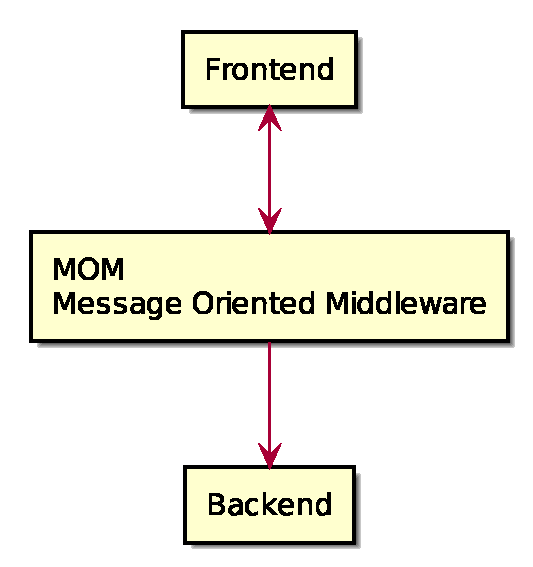
\includegraphics[height=6cm]{media/SchichtenArchitektur.eps}
    \end{figure}
\end{frame}


\section{Frontend}
\begin{frame}
    \frametitle{Frontend}
    \begin{columns}
        \begin{column}{0.48\textwidth}
            \begin{itemize}
                \item TypeScript als Programmiersprache
                \item Vue.js für UI-Komponenten
                \item Vuex für Zustandsverwaltung und unidirektionalen Datenfluss
                \item Bibliothek für STOMP oder MQTT (Verbindung zu RabbitMQ)
            \end{itemize}
        \end{column}
        \begin{column}{0.48\textwidth}
            \begin{figure}
                \centering
                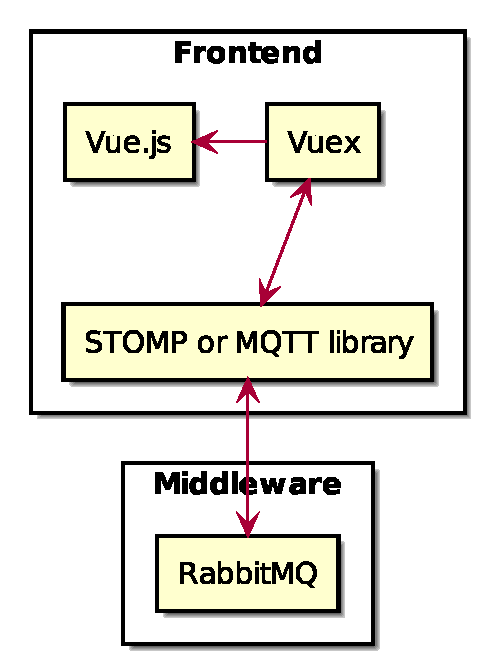
\includegraphics[height=6cm]{media/Frontend.eps}
            \end{figure}
        \end{column}
    \end{columns}
\end{frame}

\begin{frame}
    \frametitle{Vue.js}
    \begin{columns}
        \begin{column}{0.68\textwidth}
            \begin{itemize}
                \item Frontend Framework für UI-Komponenten
                \item Vergleichbar mit React (Virtual DOM, usw.)
                \item Komponenten erweitern HTML-Elemente über Direktiven
            \end{itemize}
        \end{column}
        \begin{column}{0.28\textwidth}
            \begin{figure}
                \centering
                
\includegraphics[height=3cm]{media/Vue-JS-01.eps}
            \end{figure}
        \end{column}
    \end{columns}
\end{frame}

\begin{frame}
    \frametitle{Vuex}
    \begin{columns}
        \begin{column}{0.58\textwidth}
            \begin{itemize}
                \item Ein einziger Datenspeicher als \textit{Single Source of Truth}
                \item Vergleichbar mit Redux
                \item Daten fliessen immer in eine Richtung
                \item Aktionen (User-Interaktion, Messages, usw.) verändern den Zustand, was zu einer Aktualisierung des GUI führt.
            \end{itemize}
        \end{column}
        \begin{column}{0.38\textwidth}
            \begin{figure}
                \centering
                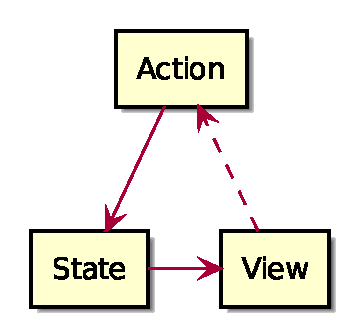
\includegraphics[height=4cm]{media/Vuex.eps}
            \end{figure}
        \end{column}
    \end{columns}
\end{frame}

\section{Message Oriented Middleware}
\begin{frame}
    \frametitle{Message Oriented Middleware}
    \begin{itemize}
        \item Übernimmt die Übermittlung und Verteilung der Nachrichten
        \item Übernimmt die Kommunikation zwischen den einzelnen Clients (Frontend und Backend)
        \item Als Message Broker wird RabbitMQ eingesetzt.
    \end{itemize}
\end{frame}

\begin{frame}
    \frametitle{RabbitMQ}
    \begin{columns}
        \begin{column}{0.68\textwidth}
            \begin{itemize}
                \item Message Broker Software für AMQP
                \item Unterstützt durch Plugins auch STOMP und MQTT über Websockets
                \item Einfaches Setup durch Docker Container
            \end{itemize}
        \end{column}
        \begin{column}{0.28\textwidth}
            \begin{figure}
                \centering
                
\includegraphics[height=3cm]{media/RabbitMQ-01.eps}
            \end{figure}
        \end{column}
    \end{columns}
\end{frame}


\section{Backend und Persistenz}
\begin{frame}
    \frametitle{Backend und Persistenz}
    \begin{itemize}
        \item In unserem Konzept wird das Dokument nur von Clients bearbeitet.
        \item Das Backend hat nur die Aufgabe den State des Dokuments zu speichern und neuen Clients zur Verfügung zu stellen.
        \item Es hört - wie alle Clients - auf der Message Queue mit und schreibt alle State Änderungen in eine MongoDB.
    \end{itemize}
    \centering
    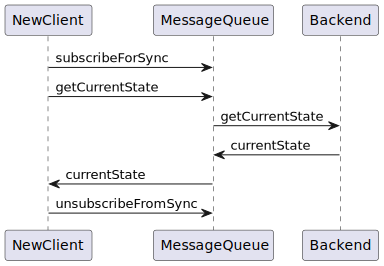
\includegraphics[height=5cm]{media/getStateFromBackend}\label{fig:Get State from Backend Diagramm}
\end{frame}


\section{Zusammenfassung}
\begin{frame}
    \frametitle{Zusammenfassung}
    \begin{figure}
        \centering
        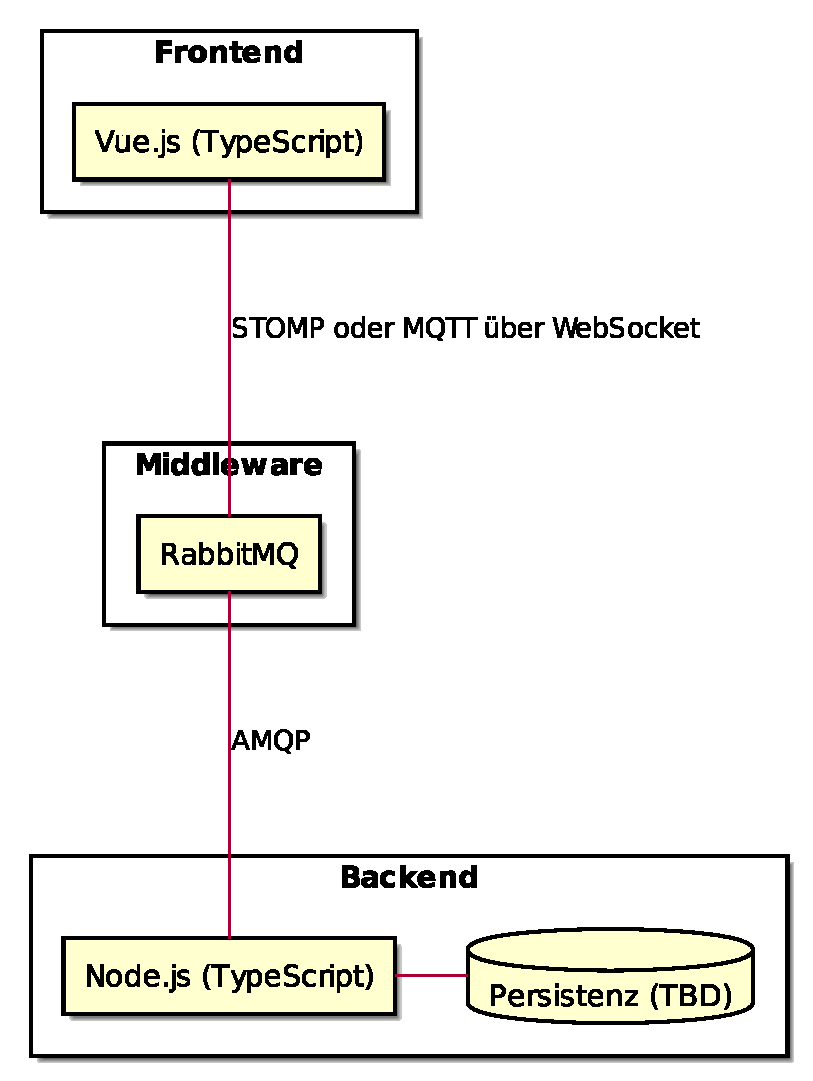
\includegraphics[height=6cm]{media/Technologien.eps}
    \end{figure}
\end{frame}

\section{Testing und Qualitätssicherung}
\begin{frame}
    \frametitle{Testing und Qualitätssicherung}
    \begin{itemize}
        \item Einsatz von Jest für Unit Tests in Frontend und Backend.
        \item Das GUI wird mit Selenium getestst, dabei wird auch ein End-To-End Test durchgeführt.
        \item Usability und Accessibility werden mit Browser Plugins von WAVE geprüft.
        \item Zum Sicherstellen einer gewissen Code Qualität wird ESLint eingesetzt.
    \end{itemize}
\end{frame}

\title{Vielen Dank für die Aufmerksamkeit}
\subtitle{Fragen?}
\author{}
\institute{}
\date{}
\begin{frame}
    \maketitle
    \thispagestyle{empty}
\end{frame}

\end{document}
